%
%
%
% ██╗    ██╗ ██████╗ ██╗████████╗███████╗██╗  ██╗
% ██║    ██║██╔═══██╗██║╚══██╔══╝██╔════╝██║ ██╔╝
% ██║ █╗ ██║██║   ██║██║   ██║   █████╗  █████╔╝
% ██║███╗██║██║   ██║██║   ██║   ██╔══╝  ██╔═██╗
% ╚███╔███╔╝╚██████╔╝██║   ██║   ███████╗██║  ██╗
%  ╚══╝╚══╝  ╚═════╝ ╚═╝   ╚═╝   ╚══════╝╚═╝  ╚═╝
%
%
%
% .##.......####...######..######..##..##.
% .##......##..##....##....##.......####..
% .##......######....##....####......##...
% .##......##..##....##....##.......####..
% .######..##..##....##....######..##..##.
%
%
%
\documentclass[8pt,american]{beamer}
\usepackage{amsmath}
\usepackage{amssymb}
\usepackage{babel}
\usepackage{float}
\usepackage[T1]{fontenc}
\usepackage{graphicx}
\usepackage[none]{hyphenat}
\usepackage[utf8]{inputenc}
\usepackage{lmodern}
\usepackage{microtype}
\usepackage{ragged2e}
\setbeamertemplate{footline}{}
\setbeamertemplate{headline}{}
\setbeamertemplate{navigation symbols}{}
\setlength{\parindent}{0pt}
\setlength{\parskip}{\medskipamount}
\usetheme{Rochester}
\usecolortheme{beetle}
\author{Marcio Woitek}
\date{\today}
\title[]{Notes on Neural Networks}

\begin{document}

\frame{\titlepage}

\section[]{Model Representation}

\begin{frame}{Model Representation}

\begin{figure}[H]
\centering
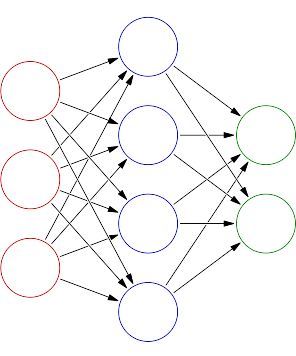
\includegraphics[height=0.8\textheight]{neural_network.png}
\caption{Basic Structure of a Neural Network}
\label{fig:neural_network}
\end{figure}

\end{frame}

\begin{frame}{Model Representation}

\begin{block}{Fundamental Ideas}
\begin{itemize}
\justifying
\item A neural network is formed by nodes or \textit{units}.
\item The units are organized in \textit{layers}.
\item There are at least two layers, the \textit{input layer} and the
  \textit{output layer}.
\item However, very often, between these layers there are
  \textit{hidden layers}.
\item In Fig.~\ref{fig:neural_network}, the red nodes form the input layer, the
  blue nodes form the hidden layer, and the green nodes form the output layer.
\item For simplicity, in the next slides, we discuss the particular case of the
  neural network in this figure.
\end{itemize}
\end{block}

\end{frame}

\begin{frame}{Model Representation}

\begin{block}{Underlying Mathematical Concepts}
\begin{itemize}
\justifying
\item First, consider the input layer.
\item We assume there are $n_{1}$ input units. In the case of
  Fig.~\ref{fig:neural_network}, we have $n_{1}=3$.
\item We denote the input values by $x_{1},x_{2},\ldots,x_{n_{1}}$.
\item There can also be an extra unit, the so-called \textit{bias unit}. Its
  value is represented by $x_{0}$. We shall set every bias unit value equal to
  1.
\item It is convenient to organize all these values in a single
  $\left(n_{1}+1\right)$-dimensional column vector:
  \begin{equation}
  \mathbf{a}^{\left(1\right)}=\begin{bmatrix}x_{0}\\
  x_{1}\\
  \vdots\\
  x_{n_{1}}
  \end{bmatrix}.
  \end{equation}
\end{itemize}
\end{block}

\end{frame}

\begin{frame}{Model Representation}

\begin{block}{Underlying Mathematical Concepts}
\begin{itemize}
\justifying
\item We can use a similar idea to represent the values related to the other
  layers.
\item To be more precise, we assume the neural network has $L$ layers.
\item Then the values associated with the $j$-th layer will be organized in a
  column vector $\mathbf{a}^{\left(j\right)}$ $\left(j=1,\ldots,L\right)$.
\item For $j\neq L$, the vector $\mathbf{a}^{\left(j\right)}$ is
  $\left(n_{j}+1\right)$-dimensional, where $n_{j}$ denotes the number of units
  in the $j$-th layer.
\item This vector has an extra dimension because the value associated with the
  bias unit of this layer is also included in $\mathbf{a}^{\left(j\right)}$.
\item However, the output layer doesn't have a bias unit. For this reason, the
  vector $\mathbf{a}^{\left(L\right)}$ is $n_{L}$-dimensional.
\end{itemize}
\end{block}

\end{frame}

\begin{frame}{Model Representation}

\begin{block}{Example of Fig.~\ref{fig:neural_network}}
\begin{itemize}
\justifying
\item As an example, we discuss the neural network in
  Fig.~\ref{fig:neural_network}.
\item Clearly, this network has $L=3$ layers.
\item Then the unit values are organized in 3 vectors,
  $\mathbf{x}=\mathbf{a}^{\left(1\right)}$, $\mathbf{a}^{\left(2\right)}$ and
  $\mathbf{y}=\mathbf{a}^{\left(3\right)}$.
\item From Fig.~\ref{fig:neural_network}, we can see that the numbers of units
  are given by $n_{1}=3$, $n_{2}=4$ and $n_{3}=2$.
\item Therefore, taking into account the values of the bias units, we can state
  the following: $\mathbf{a}^{\left(1\right)}\in\mathbb{R}^{4}$,
  $\mathbf{a}^{\left(2\right)}\in\mathbb{R}^{5}$ and
  $\mathbf{a}^{\left(3\right)}\in\mathbb{R}^{2}$.
\end{itemize}
\end{block}

\end{frame}

\section[]{Forward Propagation}

\begin{frame}{Forward Propagation}

\begin{block}{}
\begin{itemize}
\justifying
\item Next, we explain how the input values are propagated in the network.
\item Essentially, we start from the input vector
  $\mathbf{x}=\mathbf{a}^{\left(1\right)}$, and map
  $\mathbf{a}^{\left(j\right)}$ to $\mathbf{a}^{\left(j+1\right)}$ until we
  obtain the output vector $\mathbf{y}=\mathbf{a}^{\left(L\right)}$.
\item In our example, the idea is the following: first, the input vector
  $\mathbf{x}=\mathbf{a}^{\left(1\right)}$ is mapped to
  $\mathbf{a}^{\left(2\right)}$, and then this vector is mapped to
  $\mathbf{a}^{\left(3\right)}$, producing the output $\mathbf{y}$.
\item To be specific about how these mappings work, we introduce 2 vectors,
  $\mathbf{z}^{\left(2\right)}$ and $\mathbf{z}^{\left(3\right)}$.
\item In general, we introduce $L-1$ vectors $\mathbf{z}^{\left(j\right)}$,
  where $j=2,\ldots,L$.
\item We also define a set with $L-1$ functions $g^{\left(j\right)}$, where
  $j=2,\ldots,L$. The function $g^{\left(j\right)}$ is called the
  \textit{activation function} of the $j$-th layer. Notice that there isn't an
  activation function associated with the input layer.
\item To discuss our example, we consider the particular case in which all
  activation functions are the same. We denote this function by $h$.
\end{itemize}
\end{block}

\end{frame}

\begin{frame}{Forward Propagation}

\begin{block}{Activation Function}
\begin{itemize}
\justifying
\item For the activation functions, there are many choices.
\item To discuss our example, we consider the particular case in which $h$ is
  the \textit{sigmoid} or \textit{logistic function}:
  \begin{equation}
  h\left(x\right)=\frac{1}{1+\exp\left(-x\right)}.
  \label{eq:defn_sigm}
  \end{equation}
\end{itemize}
\begin{figure}[H]
\centering
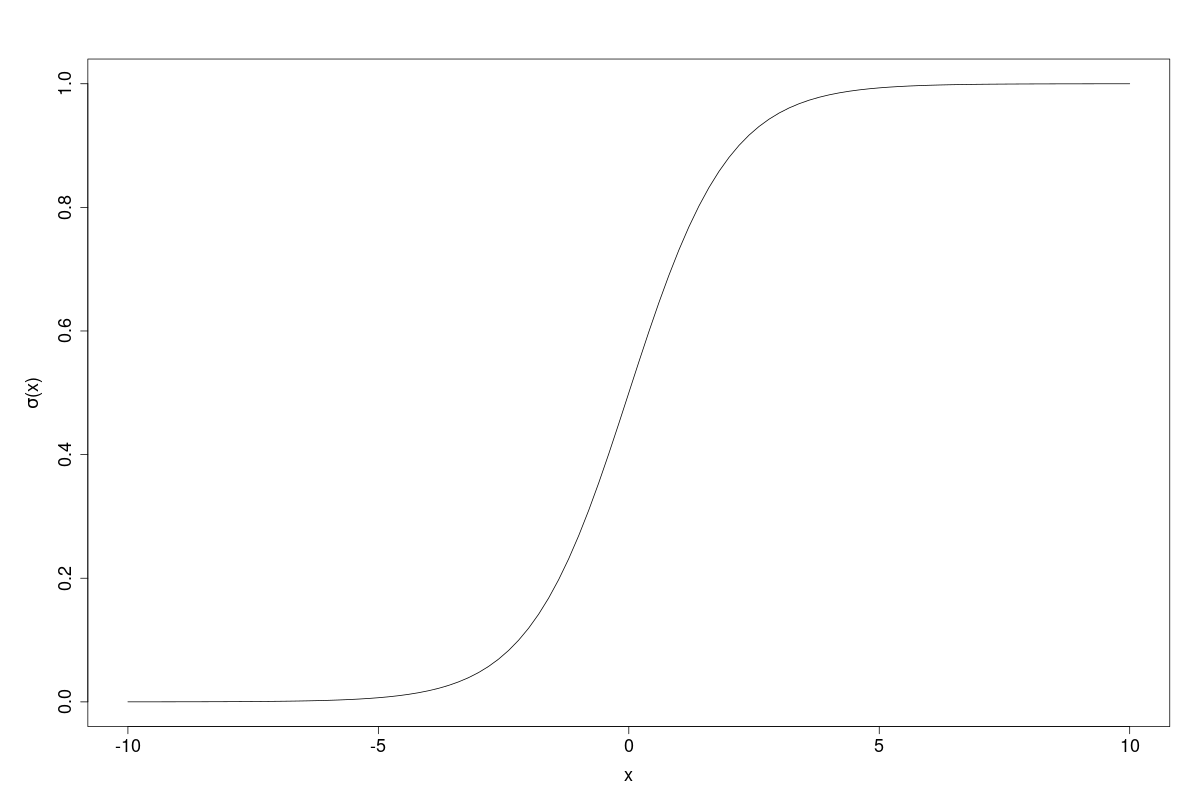
\includegraphics[height=0.4\textheight]{../r/sigmoid.png}
\caption{Graph of the sigmoid function.}
\label{fig:graph_sigm}
\end{figure}
\end{block}

\end{frame}

\begin{frame}{Forward Propagation}

\begin{block}{Forward Propagation Equations}
\begin{itemize}
\justifying
\item We continue by explaining how the vector $\mathbf{z}^{\left(j\right)}$ is
  computed from the unit values in $\mathbf{a}^{\left(j-1\right)}$.
\item We imagine all units in the $\left(j-1\right)$-th layer (including the
  bias unit) are connected to every unit in the $j$-th layer (excluding the
  bias unit).
\item Then between these layers there are $\left(n_{j-1}+1\right)n_{j}$
  connections.
\item Each of these connections has a different \textit{weight}. We will
  organize all these weights in a matrix denoted by $\Theta^{\left(j-1\right)}$.
\item The element $\Theta_{ik}^{\left(j-1\right)}$ in the $i$-th row and $k$-th
  column of this matrix is interpreted as follows: it is the weight of the
  connection between the $k$-th unit in the $\left(j-1\right)$-th layer and the
  $i$-th unit in the $j$-th layer.
\item Then the dimension of the matrix $\Theta^{\left(j-1\right)}$ is
  $n_{j}\times\left(n_{j-1}+1\right)$.
\end{itemize}
\end{block}

\end{frame}

\begin{frame}{Forward Propagation}

\begin{block}{Forward Propagation Equations}
\begin{itemize}
\justifying
\item Finally, we can write down the equations that determine the vector
  $\mathbf{z}^{\left(j\right)}$.
\item The $i$-th component of this vector is given by the \textit{weighted sum}
  of the components of $\mathbf{a}^{\left(j-1\right)}$:
  \begin{align}
  \nonumber z_{i}^{\left(j\right)}&=\Theta_{i0}^{\left(j-1\right)}a_{0}^{\left(j-1\right)}+\Theta_{i1}^{\left(j-1\right)}a_{1}^{\left(j-1\right)}+\ldots+\Theta_{i,n_{j-1}}^{\left(j-1\right)}a_{n_{j-1}}^{\left(j-1\right)}\\
  &=\sum_{k=0}^{n_{j-1}}\Theta_{ik}^{\left(j-1\right)}a_{k}^{\left(j-1\right)}.
  \end{align}
\item The last expression can be written in matrix form as follows:
  \begin{equation}
  \mathbf{z}^{\left(j\right)}=\Theta^{\left(j-1\right)}\mathbf{a}^{\left(j-1\right)}.
  \end{equation}
\item Notice that the vector $\mathbf{z}^{\left(j\right)}$ is
  $n_{j}$-dimensional.
\end{itemize}
\end{block}

\end{frame}

\begin{frame}{Forward Propagation}

\begin{block}{Forward Propagation Equations}
\begin{itemize}
\justifying
\item For $j\neq L$, to obtain the vector $\mathbf{a}^{\left(j\right)}$, we
  only need to apply the activation function $g^{\left(j\right)}$ to every
  component of $\mathbf{z}^{\left(j\right)}$, and add the bias unit of the
  $j$-th layer:
  \begin{equation}
  \mathbf{a}^{\left(j\right)}=\begin{bmatrix}a_0^{\left(j\right)}\\
  g^{\left(j\right)}\left(z_{1}^{\left(j\right)}\right)\\
  \vdots\\
  g^{\left(j\right)}\left(z_{n_{j}}^{\left(j\right)}\right)
  \end{bmatrix},
  \end{equation}
  where $a_0^{\left(j\right)}=1$. Clearly, the above vector is
  $\left(n_{j}+1\right)$-dimensional.
\item Equivalently, we can write
  \begin{equation}
  \mathbf{a}^{\left(j\right)}=\begin{bmatrix}a_0^{\left(j\right)}\\
  g^{\left(j\right)}\left(\mathbf{z}^{\left(j\right)}\right)
  \end{bmatrix}=\begin{bmatrix}1\\
  g^{\left(j\right)}\left(\Theta^{\left(j-1\right)}\mathbf{a}^{\left(j-1\right)}\right)
  \end{bmatrix}.
  \end{equation}
\end{itemize}
\end{block}

\end{frame}

\begin{frame}{Forward Propagation}

\begin{block}{Forward Propagation Equations}
\begin{itemize}
\justifying
\item As explained, we treat the vector $\mathbf{a}^{\left(L\right)}$
  differently.
\item Recall that, in this case, it isn't necessary to add the value of the
  bias unit.
\item Therefore, to compute $\mathbf{a}^{\left(L\right)}$, we only need to
  apply the activation function $g^{\left(L\right)}$ to every component of the
  vector $\mathbf{z}^{\left(L\right)}$:
  \begin{equation}
  \mathbf{a}^{\left(L\right)}=g^{\left(L\right)}\left(\mathbf{z}^{\left(L\right)}\right)=g^{\left(L\right)}\left(\Theta^{\left(L-1\right)}\mathbf{a}^{\left(L-1\right)}\right).
  \end{equation}
\item Notice that this vector is $n_{L}$-dimensional.
\end{itemize}
\end{block}

\end{frame}

\begin{frame}{Forward Propagation}

\begin{block}{Neural Network as a Composition of Mappings}
\begin{itemize}
\justifying
\item Then we have found the mappings we were looking for.
\item We can propagate the input values by using $L-1$ functions.
\item These functions are denoted by $f^{\left(j\right)}$, where
  $j=2,\ldots,L$.
\item First, we present their definition for $j\neq L$.
\item In this case, to obtain $\mathbf{a}^{\left(j\right)}$ from
  $\mathbf{a}^{\left(j-1\right)}$, we apply the function
  $f^{\left(j\right)}:\mathbb{R}^{n_{j-1}+1}\rightarrow\mathbb{R}^{n_{j}+1}$
  defined by
  \begin{equation}
  \mathbf{a}^{\left(j\right)}=f^{\left(j\right)}\left(\mathbf{a}^{\left(j-1\right)}\right)=\begin{bmatrix}1\\
  g^{\left(j\right)}\left(\Theta^{\left(j-1\right)}\mathbf{a}^{\left(j-1\right)}\right)
  \end{bmatrix}.
  \end{equation}
\item Moreover, when $j=L$, we use the function
  $f^{\left(L\right)}:\mathbb{R}^{n_{L-1}+1}\rightarrow\mathbb{R}^{n_{L}}$
  given by
  \begin{equation}
  \mathbf{a}^{\left(L\right)}=f^{\left(L\right)}\left(\mathbf{a}^{\left(L-1\right)}\right)=g^{\left(L\right)}\left(\Theta^{\left(L-1\right)}\mathbf{a}^{\left(L-1\right)}\right).
  \end{equation}
\end{itemize}
\end{block}

\end{frame}

\begin{frame}{Forward Propagation}

\begin{block}{Neural Network as a Composition of Mappings}
\begin{itemize}
\justifying
\item To make the above discussion clearer, we analyze the neural network of
  Fig.~\ref{fig:neural_network}.
\item We already know the following about this example:
\item the numbers of units are $n_{1}=3$, $n_{2}=4$ and $n_{3}=2$;
\item the unit values are organized in $L=3$ vectors,
  $\mathbf{x}=\mathbf{a}^{\left(1\right)}\in\mathbb{R}^{4}$,
  $\mathbf{a}^{\left(2\right)}\in\mathbb{R}^{5}$ and
  $\mathbf{y}=\mathbf{a}^{\left(3\right)}\in\mathbb{R}^{2}$.
\item Then, in this case, we need 2 activation functions $g^{\left(2\right)}$ and
  $g^{\left(3\right)}$. Both are single-variable real functions, since they act
  on components of vectors.
\item We use these functions to define 2 more mappings $f^{\left(2\right)}$ and
  $f^{\left(3\right)}$.
\item The function $f^{\left(2\right)}:\mathbb{R}^{4}\rightarrow\mathbb{R}^{5}$
  is defined as follows:
  \begin{equation}
  \mathbf{a}^{\left(2\right)}=f^{\left(2\right)}\left(\mathbf{x}\right)=\begin{bmatrix}1\\
  g^{\left(2\right)}\left(\Theta^{\left(1\right)}\mathbf{x}\right)
  \end{bmatrix},
  \label{eq:mapping_f2}
  \end{equation}
  where the dimension of the matrix $\Theta^{\left(1\right)}$ is
  $n_{2}\times\left(n_{1}+1\right)$, i.e., $4\times4$.
\end{itemize}
\end{block}

\end{frame}

\begin{frame}{Forward Propagation}

\begin{block}{Neural Network as a Composition of Mappings}
\begin{itemize}
\justifying
\item The function $f^{\left(3\right)}:\mathbb{R}^{5}\rightarrow\mathbb{R}^{2}$
  is defined as follows:
  \begin{equation}
  \mathbf{y}=f^{\left(3\right)}\left(\mathbf{a}^{\left(2\right)}\right)=g^{\left(3\right)}\left(\Theta^{\left(2\right)}\mathbf{a}^{\left(2\right)}\right),
  \label{eq:mapping_f3}
  \end{equation}
  where the dimension of the matrix $\Theta^{\left(2\right)}$ is
  $n_{3}\times\left(n_{2}+1\right)$, i.e., $2\times5$.
\item By using Eqs.~(\ref{eq:mapping_f2}) and~(\ref{eq:mapping_f3}), we can
  show that the output vector $\mathbf{y}$ is obtained from the input vector
  $\mathbf{x}$ by means of a composition of the mappings $f^{\left(2\right)}$
  and $f^{\left(3\right)}$:
  \begin{equation}
  \mathbf{y}=f^{\left(3\right)}\left(\mathbf{a}^{\left(2\right)}\right)=f^{\left(3\right)}\left(f^{\left(2\right)}\left(\mathbf{x}\right)\right).
  \end{equation}
\item To make this even clearer, we define a mapping
  $F:\mathbb{R}^{4}\rightarrow\mathbb{R}^{2}$ by
  \begin{equation}
  F=f^{\left(3\right)}\circ f^{\left(2\right)}.
  \end{equation}
\item Hence:
  \begin{equation}
  \mathbf{y}=F\left(\mathbf{x}\right).
  \end{equation}
\end{itemize}
\end{block}

\end{frame}

\begin{frame}{Forward Propagation}

\begin{block}{Neural Network as a Composition of Mappings}
\begin{itemize}
\justifying
\item Next, we present the general version of the above idea.
\item In general, we consider the composition of the $L-1$ functions
  $f^{\left(j\right)}$, where $j=2,\ldots,L$.
\item This allows us to write the output vector as
  \begin{equation}
  \mathbf{y}=F\left(\mathbf{x}\right),
  \end{equation}
  where the mapping $F:\mathbb{R}^{n_{1}+1}\rightarrow\mathbb{R}^{n_{L}}$ is
  defined by
  \begin{equation}
  F=f^{\left(L\right)}\circ\cdots\circ f^{\left(3\right)}\circ f^{\left(2\right)}.
  \end{equation}
\item The most important conclusion from this discussion is the following:
\item \textbf{the propagation of the input values is implemented mathematically
  by means of a composition of mappings}.
\end{itemize}
\end{block}

\end{frame}

\end{document}
